\PassOptionsToPackage{utf8}{inputenc}
\documentclass{bioinfo}

\usepackage[draft]{hyperref}
\usepackage{makecell}
\usepackage{comment}
\usepackage{subcaption}
\usepackage{algorithm2e}
\usepackage[usenames,dvipsnames]{xcolor}


\SetAlgoLined
\SetKwProg{MyStruct}{Struct}{ contains}{end}

\newcommand{\vocab}{\textbf}
\newcommand{\red}[1]{{\textcolor{Red}{#1}}}
\newcommand{\FIXME}[1]{\red{[FIXME: #1]}}

\def\labelitemi{--}

\copyrightyear{XXXX} \pubyear{XXXX}

\access{Advance Access Publication Date: Day Month Year}
\appnotes{Genome Analysis}

\begin{document}
\firstpage{1}

\subtitle{Genome Analysis}

\title[short Title]{ODGI: understanding pangenome graphs}
\author[Guarracino, Heumos \textit{et~al}.]{
Andrea Guarracino\,$^{\text{\sfb 1} \dagger}$,
Simon Heumos\,$^{\text{\sfb 2} \dagger}$,
Sven Nahnsen\,$^{\text{\sfb 2}}$,
Pjotr Prins\,$^{\text{\sfb 3}}$,
and Erik Garrison\,$^{\text{\sfb 3}*}$
}

\address{
$^{\text{\sf 1}}$University of Tor Vergata, Rome, Italy \\
$^{\text{\sf 2}}$Quantitative Biology Center (QBiC), University of T\"ubingen, T\"ubingen, Germany, 72076 \\
$^{\text{\sf 3}}$University of Tennessee Health Science Center, Memphis, TN, USA
}

\corresp{$^\ast$To whom correspondence should be addressed. \\
$^\dagger$Contributed equally.}

\history{Received on XXXXX; revised on XXXXX; accepted on XXXXX}

\editor{Associate Editor: XXXXXXX}

% XXX key message of the paper is that we have collected a set of algorithms that enable easy use of pangenome graphs for investigating biology

\abstract{
\textbf{Motivation:} Pangenome graphs provide a complete representation of the mutual alignment of collections of genomes.
These models offer the opportunity to study the total genomic diversity of a population, including structurally complex regions.
However, analyzing hundreds of gigabase-scale genomes using pangenome graphs is difficult and not well-supported by existing tools.
%In addition, vertebrate genomes present highly repetitive regions which increase the complexity of the analysis.
Hence, fast and versatile software is required to ask intricate questions of such data in an efficient way. \\
\textbf{Results:} Here we present ODGI, a new suite of tools that implements scalable algorithms and has an efficient in-memory representation of DNA variation graphs. ODGI includes tools for detecting complex regions, extracting loci, removing artifacts, exploratory analysis, manipulation, validation, and visualization. Its fast parallel execution facilitates routine pangenomic tasks as well as pipelines that can quickly answer complex biological questions of gigabase-scale pangenome graphs. \\
%ODGI supports graphs in the Graphical Fragment Assembly format version 1 (GFAv1).
%The tools scale efficiently to large collections of eukaryotic genomes, allowing users to work easily with pangenome graphs of tens to thousands of large genomes while maintaining fast execution runtime and low memory overhead.
\textbf{Availability:} ODGI is under the MIT license. Source code can be downloaded from \url{https://github.com/pangenome/odgi} while the documentation is available at \url{https://odgi.readthedocs.io}.
ODGI can be installed via Bioconda \url{https://bioconda.github.io/recipes/odgi/README.html} or Guix \url{https://github.com/ekg/guix-genomics/blob/master/odgi.scm}. \\
\textbf{Contact:} \href{egarris5@uthsc.edu}{egarris5@uthsc.edu} \\
\textbf{Supplementary information:} Supplementary data are available at \textit{Bioinformatics} online.
}

\maketitle

\section{Introduction}

A pangenome models the full set of genomic elements in a given species or clade \citep{cpang2018,Eizenga_2020}.
In contrast to reference-based approaches which relate sequences to a single genome, these data structures encode the mutual relationships between all the genomes represented.
In pangenome graphs \citep{Paten:2017}, homologous regions between genomes are compressed into a single representative model of all alleles present in the pangenome.
These flexible models let us encode any kind of variation, allowing the generation of comprehensive data systems on which to base analyses of genome evolution.
Although these structures are of clear utility to researchers \citep{cpang2018}, and have been the focus of numerous applications in read mapping \citep{Garrison:2018,Baaijens_2019,Hickey:2020,Sibbesen_2021}, we observe that the community lacks a toolset specifically focused on graph manipulation and interrogation.

The Human Pangenome Reference Consortium (HPRC) and Telomere-to-Telomere (T2T) consortium \citep{Miga:2020, Logsdon_2021, Nurk_2021} have recently demonstrated that high-quality \textit{de novo} assemblies can be routinely generated from third-generation long read sequencing data.
We anticipate that in the near future, studies will frequently begin from assemblies of similar quality, leading to demand for methods that allow us to create and explore pangenomes.
Pangenome graphs are a natural model to support these kinds of analyses, but studies based on pangenome graphs are difficult due to a lack of downstream tools and standard workflows.

Here, we present the Optimized Dynamic Genome/Graph Implementation (ODGI) toolkit, a pangenome graph interrogation and transformation system specifically built to handle the data scales encountered when working with pangenomes built from hundreds of haplotype-resolved genomes.
ODGI provides a set of standard operations on the pangenome variation graph data model, generalizing ``genome arithmetic'' concepts like those found in BEDTools \citep{Quinlan_2010} to work on genome graphs, and providing new operations, such as visualizations, sorting, and liftover projections critical to understanding and exploiting pangenome graphs.

%Tools in ODGI operate on an efficient dynamic HandleGraph model \citep{Eizenga_2020_BX}.
%Algorithms written against this abstract API can be applied to the graph.% applies algorithms based on the HandleGraph API.
%This common API lets us reuse and and extend algorithms shared with the VG toolkit (VG) \citep{Garrison:2018}.
%We specifically develop new methodsfocused on problems encountered when building pangenome graphs at the scale of vertebrate populations.
%To ease interactive use, the majority of the ODGI tools are implemented in an index-free manner, avoiding the need to create index structures at each step of complex graph processing pipelines.
%Thanks to ODGI's efficient path representation, its tools can work with variation graphs with highly complex regions.
%This eliminates one of the major bottlenecks when working with very large and deep variation graphs, and allows researchers to build and understand graphs of previously-inaccessible complexity and scale.


%\footnote{\url{https://humanpangenome.org/} (accessed Oct 2021)}
%\footnote{\url{https://sites.google.com/ucsc.edu/t2tworkinggroup/home} (accessed Oct 2021)}.

\section{Model}

A pangenome graph is a sequence model that encodes the mutual alignment of many genomes \citep{Garrison_2019_thesis,Eizenga_2020}.
In the variation graph, $V = (N, E, P)$, nodes $N = n_1\ldots n_{|N|}$ contain sequences of DNA.
Each node $n_i$ has an identifier $i$ and an implicit reverse complement $\bar{n_i}$, and a node strand $s$ corresponds to one such orientation.
Edges $E = e_1\ldots e_{|E|}$ represent ordered pairs of node strands: $e_i = ( s_a, s_b )$.
Paths $P = p_1\ldots p_{|P|}$ describe walks over node strands: $p_i = s_1 \ldots s_{|p_i|}$.
When used as a pangenome graph, $V$ expresses sequences, haplotypes, and annotations as paths.
%The utility of the variation graph model lies in its lossless representation of genomes and their alignment.
By containing both the sequences and information about their relative variations, the variation graph provides a powerful foundation for many bioinformatic applications.

Such a graph can be constructed by multiple sequence alignment \citep{Lee_2002,Grasso_2004}, but the resulting partially-ordered graph cannot represent complex variation like inversions and cycles that occur at structural scales in genomes.
General approaches to building pangenome graphs transitively reduce an alignment between sequences to an equivalent, labeled sequence graph \citep{Kehr_2014,Garrison_2019_thesis}.
Current methods to build these graphs are still in development \citep{Li:2020,Armstrong:2020,pggb}, but they have largely settled on a common data model, represented in the Graphical Fragment Assembly (GFA) format \citep{GFA}).
%The improvement of these methods depends on tools that allow us to investigate
This standardization supports the development of a reference set of tools that operate on the pangenome graph model.
%The need to understand the graphs made by these methods motivates it.
We require such a toolkit to understand the graphs made by these methods.

%The improvement of these approaches depends on scalable tools for understanding pangenome graphs, a need that our work responds to.

%As a toolkit for understanding these graphs, ODGI

%A more general approach is to build the graph from an alignment between sequences.
%We first transitively collapse characters in the input sequences that align together into single character in the output genome
%By projecting input sequences through this transformation, we obtain paths that losslessly encode the original sequences, but in the space of the graph \citep{Garrison_2019_thesis}.
%Methods to build such graphs are in active development, and here we focus on graphs built with the PanGenome Graph Builder pipeline \citep{pggb}, a process that converts an input pangenome (in FASTA) into a combined graphical model (in the Graphical Fragment Assembly (GFA) format \citep{GFA}).

\section{Implementation}

%ODGI is designed to build and modify paths in parallel, keeping its representation in memory efficient.
The ODGI toolkit builds on existing approaches to efficiently store and manipulate variation graphs \citep{Garrison:2018}.
%It implements the \textsc{HandleGraph} model \cite{Eizenga_2020_BX}.
Similar to other efficient libaries presenting the \textsc{HandleGraph} model \citep{Eizenga_2020_BX}, ODGI's implementation rests on three key properties which hold for most pangenome variation graphs:

\begin{enumerate}
\item They are relatively sparse, with low average node degree.
\item They can be sorted so that most edges go between nodes that are close together in the sort order.
\item Their embedded paths are locally similar to each other.
%We incorporate concepts first introduced in the dynamic version of the Graph BWT \citep{Siren:2020} (GBWT), a scalable implementation of the graph extension of the positional Burrows-Wheeler transform \citep{Durbin_2014}.
\end{enumerate}

These properties are used to build efficient dynamic variation graph data structures \citep{Siren:2020,Eizenga_2020_BX}.
Sparsity (1) allows us to encode edges $E$ using adjacency lists rather than matrices or hash tables.
The local linear structure of the graph (2) lets us assign node identifiers that increase along the linear components of the graph, which supports a compact storage of edges and path steps as relativistic (usually small) differences rather than absolute (always large) integer identifiers.
Path similarity (3) allows us to write local compressors that reduce the storage cost of collections of path steps.
%\FIXME{without a figure we may lose the reader here a little} -- see algorithm 1

%Here, we build on this work and focus on issues that have arisen during our recent work on the Human Pangenome.
ODGI improves on prior efforts, based on issues that arose during our work with high-quality assemblies that cover almost all parts of the genome \citep{Logsdon_2021,Nurk_2021}.
%A key design objective, motivated by experience working with graphs built from high quality eukaryotic genome assemblies, is to support graphs with very high path depth.
For example, we find that it is necessary to support graphs that have regions of very high path depth.
Such motifs can occur in collapsed repeat structures generated by ambiguous sequence homology relationships in repeats found in the centromeres and other segmental duplications.
If we cannot process such regions, we have only two options: 1) we can remove these regions, or 2) we can leave them unaligned. However, neither of these solutions allows us to investigate their biological features.
To seamlessy represent such difficult regions, we follow an approach implemented in the dynamic version of the Graph BWT (GBWT) \citep{Siren:2020}, and built a node-centric, dynamic, compressed model of the paths.
This design supports node-local modification and update of the graph, which lets us build and transform the model in parallel.

We store the graph in a vector of node structures, each of which presents a node-local view of the graph sequence, topology, and path layout.
Expressed in terms of the variation graph $V$, ODGI's core $Node$ structure includes a decoder that maps the neighbors of each node to a dense range of integers.
For a given node $i$ and neighbor $j$, the decoder itself does not store the $id$s of $j$, but rather a compact representation of the relative difference between the node ids: $\delta = Node_i.id - Node_j.id$.
This keeps even the size of the encoding small, per common variation graph property (2).
We define the edges and path steps traversing the node in terms of this alphabet of $\delta$'s.
The structures in Algorithm \ref{alg:structs} describes our encoding.

\begin{algorithm}
\MyStruct{Node}{
    \textbf{id} $\in \mathbb{N}$ \tcp{an identifier}
    \textbf{lock} \tcp{atomic locking primitive}
    \textbf{sequence} $= [$A$|$T$|$G$|$C$|$N$]*$ \tcp{DNA}
    \tcp{bit-packed vector of edges}
    \textbf{edges} $= (x_i,x_j)* : (i, j) \in [1\ldots \Sigma]^2$ \\
    \tcp{bit-packed vector of id deltas}
    \textbf{decoding} $x_1 \ldots x_{\Sigma} \in \mathbb{N}^\Sigma$ \\
    \tcp{bit-packed vector of path steps}
    \textbf{path\_steps} $[Step_1 \ldots Step_n]*$
}
\MyStruct{Step}{
    \textbf{path\_id} $\in \mathbb{N}$ \tcp{the path's global id}
    \textbf{is\_rev} $\in ( 0, 1 )$ \tcp{the step orientation}
    \textbf{is\_start} $\in ( 0, 1 )$ \tcp{if first step in path}
    \textbf{is\_end} $\in ( 0, 1 )$ \tcp{if last step in path}
    \textbf{prev\_$\delta$} $\in [1\ldots \Sigma]$ \tcp{$\delta$-encoded previous node}
    \textbf{prev\_rank} $\in \mathbb{N}$ \tcp{step rank on previous node}
    \textbf{next\_$\delta$} $\in [1\ldots \Sigma]$ \tcp{$\delta$-encoded previous node}
    \textbf{next\_rank} $\in \mathbb{N}$ \tcp{step rank on next node}
}
\caption{ODGI's relativistically-packed $Node$ structure and the $Step$ structure used to represent the paths as doubly-linked lists.}
\label{alg:structs}
\end{algorithm}


Each structure contains the sequence of the node ($Node_i.sequence$), its edges in both directions ($Node_i.edges$), and a vector of path steps that describes the previous and next steps in paths that walk across the node ($Node_i.path\_steps$).
%As in the GBWT, to compress the encoding, we encode path steps using a local alphabet that maps the N neighbours of the node into the range $1\ldots N$.
%To further save space, node deltas, rather than IDs, are stored in this alphabet.
%The delta between two nodes is defined as their distance in the graph vector (i.e., the difference between the node offsets).
For efficiency, $Node_i.sequence$ is stored as a plain string, while the $edges$ and $path\_steps$ are stored using a dynamic succinct integer vector that requires $O(2nw)$ bits for the edges and $O(5nw)$ bits for the path steps, where $n$ is the number of steps on the node, and $w$ is $\approx log_2(n)$ \citep{prezza2017framework}.

To allow edit operations in parallel, each node structure includes a byte-width mutex $lock$.
All edit operations on the graph must touch at most two $Node$ structs at a time (both edge and path step representations are doubly-linked).
To avoid deadlocks, we acquire the node locks in ascending $Node.id$ order and release them in desceding order.
In addition to node-local features of the graph, we must maintain some global information.
Specifically, we record the start and end of paths, as well as a name to path id mapping in lock-free hashtables.
The use of lock-free hashtables lets us avoid a global lock when looking up path or graph metadata, which would quickly become a bottleneck during parallel operations on the graph.
By avoiding global locks, we implement many of the operations in ODGI using maximum parallelism available.
This ``atomic'' approach to edit operations on the graph is key to enable our methods to scale to the largest genome graphs that we can currently build.

\begin{comment}
%\subsection{Core functionality}

Variation graphs are commonly represented by a subset of version 1 of the Graphical Fragment Assembly format (GFAv1): odgi build and odgi view allow to convert graphs from GFA to ODGI format and vice versa, respectively.
In the variation graph model, paths have to respect the graph’s topology: this can be verified with odgi validate, to ensure no errors in the input or edited graphs.

Applying odgi stats, users can retrieve metrics describing the graph properties, such as the number of nodes, edges, paths, and graph length.
ODGI also offers more advanced tools for interrogating the graphs. odgi bin summarizes the path information into bins of specified size, enabling a summarized view of gigabase scale graphs.
odgi depth returns the node depth as defined by query criteria, allowing users to detect the complex regions in the graph due to sequences with highly identical repeats.
Complex motifs can be also detected with odgi degree, which returns the node degree as defined by query criteria.
High degree nodes are the mirror of misassemblies or problems in the pangenome building, making the tool useful for debugging the process as well.

ODGI allows edit operations on the graphs.
Cycles in the graph complicate downstream analyses: odgi break removes the cycles, reducing the complexity of the graph topology.
odgi groom removes spurious inverting links by exploring the graph from the orientation supported by most paths.
To enable efficient sequence alignment against the graph, long nodes can be divided into shorter nodes at a maximum requested size using odgi chop.
Partial order alignment, which consists of aligning sequences against a directed acyclic graph (DAG), is frequently used in pangenome building pipelines, but the current implementations return DAGs with 1-bp long nodes; odgi unchop allows joining nodes that can be merged without changing the graph topology, nor the embedded sequences, obtaining an equivalent, but more compact, representation of the graph.

Pangenome graphs can embed multiple chromosomes as separated connected components (inter-chromosomal structural variants would join the components into bigger ones).
odgi explode separates the connected components in different ODGI format files, while odgi squeeze allows merging multiple graphs into the same ODGI format file, preventing node ID collisions.
odgi extract allows extracting specific subregions of the graph as defined by query criteria, thereby simplifying the downstream analyses and reducing the resources to work only with the extracted region.

In variation graphs the coordinates are provided by the embedded path sequences.
Indeed, the node IDs are not meant to be stable. odgi position finds, translates, and liftovers graph and path positions between different graphs by exploiting their shared path sequences (Figure 1.B).
\end{comment}

\begin{comment}
key message of the paper is that we have collected a set of algorithms that enable easy use of pangenome graphs for investigating biology
-> build model solves problem of working with big graphs in memory
-> view (convert to GFA) & paths solve problem of exporting basic features of the graph (e.g. paths)
-> stats (understand basic size / structure) & bin & degree & depth solves problem of understanding the overall structure and size of the graph
-> sort (groom) & layout solves problem of finding latent structure in the pangenome
-> viz & draw provides a human-viewable readout of the graph
-> chop & unchop & squeeze & break & prune & explode lets us break apart or combine the graph nodes and topology
-> position & tips & untangle (jaccard based coordinate conversion) provides a way to map coordinates between any genomes in the graph (e.g. liftover!)
-> extract lets us pull out specific regions of the graph based on path ranges, nodes and positions
\end{comment}

\begin{figure*}[ht!]
  %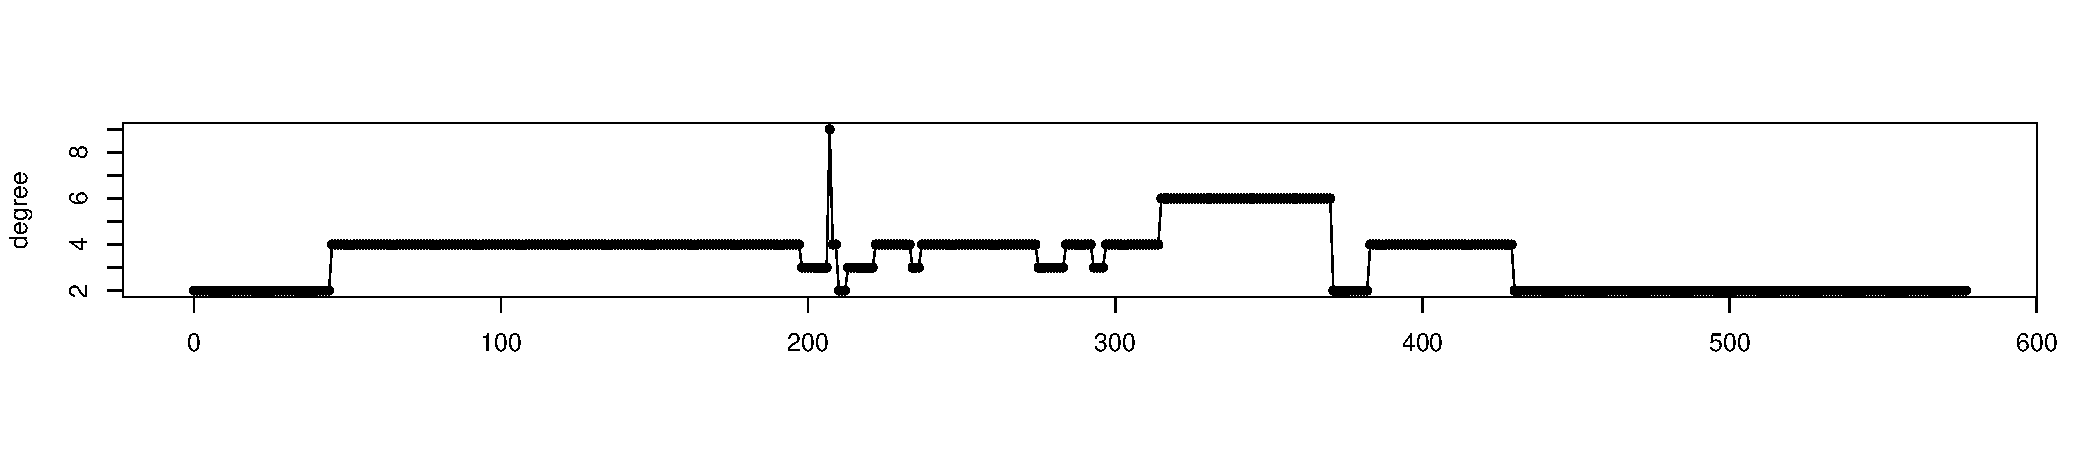
\includegraphics[width=\linewidth,trim=+.225cm 0 +.425cm +2cm]{fig/metrics/chr4_HTT_chm13_degree_w1_bed.pdf}  
  \includegraphics[width=\linewidth]{fig/odgi_tools.pdf}
  \caption{Methods provided by ODGI (in black) and their supported input and output data formats (in brown).}
  \label{fig:operations}
\end{figure*}


\section{Results}

ODGI provides a set of first-order interrogative and manipulative operations on pangenome graphs.
We have established these tools to support our exploration of graphs built from hundreds of large eukaryotic genomes.
They are practical and able to work with high levels of graph complexity, even with regions of very high path depth (10$^5$ to 10$^6$-fold coverage).
ODGI's tools cover common operations that we have found to be essential when working with these complex biological models:

\begin{itemize}
\item \textit{odgi build} constructs the ODGI data model from GFA (\S\ref{sec:build}).
\item \textit{odgi view} converts the graph into standard text formats (\S\ref{sec:text}).
\item \textit{odgi stats} provides numerical properties of the graph (\S\ref{sec:text}).
\item \textit{odgi matrix} derives the pangenome matrix (\S\ref{sec:text}).
\item \textit{odgi paths} lists and extracts paths in FASTA (\S\ref{sec:text}).
\item \textit{odgi flatten} converts the graph to FASTA and BED (\S\ref{sec:text}).
\item \textit{odgi extract} subsets the graph based on path ranges (\S\ref{sec:extract}).
\item \textit{odgi chop} breaks long nodes into shorter ones (\S\ref{sec:edit}).
\item \textit{odgi unchop} combines redundant nodes (\S\ref{sec:edit}).
\item \textit{odgi explode} breaks the graph into connected components (\S\ref{sec:edit}).
\item \textit{odgi squeeze} unifies disjoint graphs (\S\ref{sec:edit}).
\item \textit{odgi prune} removes complex regions (\S\ref{sec:edit}).
\item \textit{odgi viz} provides a scalable linear visualization of the graph (\S\ref{sec:viz}).
\item \textit{odgi draw} renders a 2D image of the graph (\S\ref{sec:viz}).
\item \textit{odgi position} lift coordinates between paths and graph positions (\S\ref{sec:untangle}).
\item \textit{odgi untangle} deconvolutes paths relative to a reference (\S\ref{sec:untangle}).
\item \textit{odgi sort} orders the graph with sorting pipelines (\S\ref{sec:sort}).
\item \textit{odgi layout} establishes a 2D layout using SGD (\S\ref{sec:sort}).
\item \textit{odgi depth} describes path depth over graph and path positions (\S\ref{sec:metrics}).
\item \textit{odgi degree} describes node degree over graph and path positions (\S\ref{sec:metrics}).
\item \textit{odgi tips} finds path end points relative to a reference (\S\ref{sec:metrics}).
\end{itemize}

Each tool focuses on a small set of related operations.
Most read or write the native ODGI format (`og' extension) (Figure \ref{fig:operations}) and work with standard text based data formats common to bioinformatics.
This supports the implementation of flexible, composable, graph processing pipelines based on a common data type.
While the pangenome graph is a first-class entity in ODGI, we focus on the embedded paths to provide a universal coordinate system.
By considering all paths in the graph as potential reference or query sequences, we make the graph invisible to downstream tools that operate on collections of sequences (e.g. bedtools, samtools, aligners).
This approach benefits from the information in the graph without strongly embedding our methods in this difficult new research context.
%ODGI provides methods that empower ``legacy'' toolsets.

%we focus on common reference-based data formats like BED and PAF to input and output information from the graph.


%To further our understanding of these graphs, we have developed a set of methods that let us inspect and manipulate them.

%We begin with a set of HandleGraph-based algorithms first establish in the VG toolkit \citep{Garrison:2018}.
%These include algorithms for graph traversal, partition-finding, $k$-mer and character enumeration, sorting, and pruning.
%Unlike VG, we provide no methods to construct graphs, map reads to the graph, or derive variants.



%To our knowledge, these methods are the first to trivially scale to operate on large base-level graphs of this type.

%To foster a high-level understanding of large graphs, we pursue a novel approach to visualization.
%ODGI provides a linear-time 1D visualization that easily renders gigabase-scale pangenomes in a human-interpretable format suitable for understanding the topology and genome releationships in the pangenome graph.
%A similar 2D visualization is more costly to compute, but similarly provides linear-time scaling, allowing us to apply it to large pangenomes.
%This removes a major bottleneck in

%Subsetting operations allow us to zoom in on particular genes or regions of interest for more precise examination.

%We extract key information about the graph using its paths as a pangenome reference system.

%We find that, to understanding relationships between sequences and positions in pangenome graphs, we must use context mapping to ``untangle'' complex regions found in VNTRs, segmental duplications, and centromeric repeats.
%This approach lets use pangenome graphs as a foundation for universal liftover between any two sets of sequences in the graph.



%It supports interrogation of the graph for basic dimensional properties, positional and path-related queries, and visualization in one-dimension (1D) and two-dimensions (2D).
%ODGI also supports operations on the graph such as subset, subdivide, break, combine, normalize, or order its components, nodes, and paths.
%Most of the tools are designed to be applied together, piping the output of one tool into the next, thereby preventing the creation of intermediate files, and reducing the number of IO operations.


\subsection{Building the \textsc{ODGI} model}
\label{sec:build}

% erik

% build
We begin by transforming the storage model of the GFA format (in which nodes, edges, and paths are described independently) into the ODGI node-centric encoding with \textit{odgi build}.
This construction step can present a significant bottleneck, in particular as the size of the path set of the graph increases.
The ODGI data structure (Algorithm \ref{alg:structs}) allows algorithms that build and modify the graph to operate in parallel, without any global locks.
In \textit{odgi build}, we initially construct the node vector in a serial operation that scans across the input GFA. Then, in serial, we add edges in the $Node.edges$ vectors of pairs of nodes. Finally, we create paths in serial, and extend them in parallel by obtaining mutex $Node.lock$ for pairs of nodes and by adding the path step in their $Node.path\_steps$ vectors.
This parallelism speeds ODGI model construction by many-fold when testing against graphs built by the HPRC (TODO).

%Figure: encoding model as a cartoon --  HTT exon 1 as tiny example graph (maybe)

\subsection{Converting to standard text formats}
\label{sec:text}

% pjotr & andrea

% view / paths
Allows us to export basic data of the graph (genomes and graph structure).

\textit{odgi view} can output GFA and internal graph representations \\
\textit{odgi stats} outputs statistics in TSV or YAML. \\
\textit{odgi bin} can output JSON. \\
\textit{odgi degree/position/depth/untangle/tips} can output BED. \\
\textit{odgi untangle} outputs PAF.

Figure: .dot showing the relationship between all the tools and the data formats we use.

\subsection{Extracting regions of interest}
\label{sec:extract}

% andrea (?)

% extract
Pangenome graphs are very large, but we often only want to work with a small portion (e.g. a single gene).
We can extract such regions using coordinates on the paths in the graph to guide us.

Figure showing extraction process---either schematic or ``real''.

\subsection{Editing the graph structure}
\label{sec:edit}

% andrea (?)

% chop / unchop / squeeze / break / prune / explode
These are commonly-needed basic operations on the topology of the graph.


\subsection{Visualizing pangenome graphs}
\label{sec:viz}

% andrea (viz) & erik (draw)

% interesting that we don't go base-level at all... we use vg for that, or STM

Pangenome graph visualization is one of the first steps to gain insight into the mutual relationship between the sequences and their variation.
\textit{odgi viz} and \textit{odgi draw} provide scalable ways of generating human-viewable pictures of the high-level structure of the graph.

\textit{odgi viz} offers a binned, linearized rendering in 1 dimension (1D).

% Explain odgi viz's visualization

However, complex, nonlinear graph structures are difficult to display and interpret in a convenient low number of dimensions.
To overcome such a limitation, \textit{odgi viz} supports multiple visualization modes, making it easy to grasp the properties of the graph and its complexity.

% Explain odgi viz's color by path position
% Explain odgi viz's color by strandness
% Explain odgi viz's color by coverage

\textit{odgi draw} extends the visualization in 2 dimensions (2D), taking in input the layouts built by \textit{odgi layout}.

% Explain odgi draw's visualization

Figure here with 1D + 2D vizs.

\subsection{Untangling and navigating the pangenome with path-based coordinates}
\label{sec:untangle}

% erik

The key data in a pangenome graph is a representation of the alignment (or homology) relationships between sequences in the pangenome.
Navigating and understanding the graph requires coordinate systems that we can use to link other data into the graph model, and thus to all genomes in the pangenome.
Primarily, ODGI uses the embedded pangenome sequences to provide a set of coordinates in a standard, 1D format.e
These coordinates depend on the sequences, and are graph-independent.
Our for positional conversion (\textit{odgi position}), annotation liftover (\textit{odgi untangle}), subgraph extraction (\textit{odgi extract}), visualization (\textit{odgi viz}), path depth (\textit{odgi depth}), and graph complexity measurement (\textit{odgi degree}) can all operate on coordinates of paths in the graph.

For understanding the large-scale organization of the graph, we benefit from an even simpler coordinate system.
To provide a universal coordinate space for the graph, we project its nodes into a low-dimensional space (in practice, 1 or 2 dimensions) by learning the projection via a HOGWILD! \citep{niu2011hogwild}, path-guided stochastic gradient descent (PG-SGD) layout algorithm that adapts SGD-based drawing to pangenome graphs \citep{zheng2018graph}.
This approach updates node relative positions to best-match their distance in the paths running through the graph.
Based on this projection, we can trivially generate 1D and 2D visualizations.
We can also detect regions whose layout is distorted, and which thus may represent structural variation or assembly error.
ODGI can project vector and matrix representations of the graph relative to these learned coordinate spaces.

In addition to these projections, we use the paths in the graph to provide a universal coordinate space.
It also supports several kinds of ``lift-over'' of coordinates between different genomes.
These allow for the direct translation of single coordinates and ranges, in an interactive way.
And, they let us extract a pairwise 1:many alignment between a given set of ``query'' sequences and a given set of ``target'' or reference sequences.
This lets us convert the graph to lift-over maps compatible with standard software for projecting annotations and alignments from one genome to another.



% position / tips
% untangle (this follows on the jaccard graph mapping concepts in the previous section}
%The graph is a model of an alignment of many genomes.
%We can use coordinates in any genome to refer to it, but this requires a few basic operations ...
%Obtaining unambiguous mappings between different genomes requires the use of a new kind of graph based mapping (path graph jaccard).

Figure showing the untangling of C4 ?
Figure showing tips over a single human chromosome from HPRC.

\subsection{Sorting the pangenome graph topology}
\label{sec:sort}

% simon

% sort / layout / NO tension! We keep that for the sorting paper

% Allows us to understand the sparse structures typically found in pangenome graphs.

%Pangenome graphs built from raw sets of alignments may have complex structures which can introduce difficulty in downstream analyses. Uncovering their latent topology allows us to understand their typical sparse structures.

\textit{odgi sort} offers multiple sorting algorithms to find the best node order in one dimension. Most notably, nodes can be sorted topologically, randomly, by breaking cycles in the graph, by grooming, or by using a novel path-guided stochastic gradient descent (PG-SGD) algorithm.
The latter one exploits the biological information in the paths for sorting the nodes.
Combining a series of sorts can mitigate the weaknesses of individually applied sorting algorithms.
%In Figure \textbf{\textit{TODO MHC wgg.85}}, a comparison of an unsorted human pangenome MHC graph and a sorted one are displayed.

%For the establishment of a layout in two dimensions \textit{odgi layout} applies a 2D adjusted PG-SGD algorithm. A calculated layout can be visualized statically with \textit{odgi draw} (see Figure \textit{\textbf{TODO MHC wgg.85}}) or interactively explored with the in-development \textit{gfaestus}\footnote{\url{https://github.com/chfi/gfaestus}}.

\subsection{Obtaining metrics of the pangenome graph}
\label{sec:metrics}

% simon
% HTT exon1
% Only chr8 longs if I can't produce someting nice

% stats / multiQC / bin / degree / depth

% Solves the problem of understanding the overall structure, size, and features of the graph and its sequences.


Graphs statistics provide alternative ways to gain insight into pangenomes complexity revealing the overall structure, size, and features of a graph and its sequences.

Applying \textit{odgi stats}, users can retrieve metrics describing the graph properties, such as the number of nodes, edges, paths, and graph length.
MultiQC's \citep{Ewels_2016} ODGI module\footnote{\url{https://multiqc.info/docs/\#odgi} (accessed Oct 2021)} provides an interactive way to comparatively explore the statistics of an arbitrary number of graphs.
ODGI also offers more advanced tools for the interrogation of the graphs. \textit{odgi bin} summarizes the path information into bins of a specified size, enabling a summarized view of gigabase scale graphs.
This concept found its way into the pangenome graph ontology \cite{Yokoyama2020}. \textit{odgi depth} returns the node depth as defined by query criteria, allowing users to assess the complexity of regions in the graph.
Collapsed sequences with highly identical repeats indicate intricate loci.
Complex motifs can be also detected with \textit{odgi degree}, which returns the node degree as defined by query criteria.
High degree nodes can be the mirror of variation, misassemblies, or problems in the pangenome building, making the tool useful for validation.
In Fig. \ref{fig:metrics}, the characteristics of a 90 haplotypes human pangenome graph of the exon 1 huntingtin gene \citep{Sathasivam2013,Neueder2017} (\textit{HTTexon1}), obtained with the ODGI metrics tools, are shown.

\begin{figure}[ht!]
    \begin{subfigure}{\linewidth}
        \caption{}
        \centering
        % include first image
        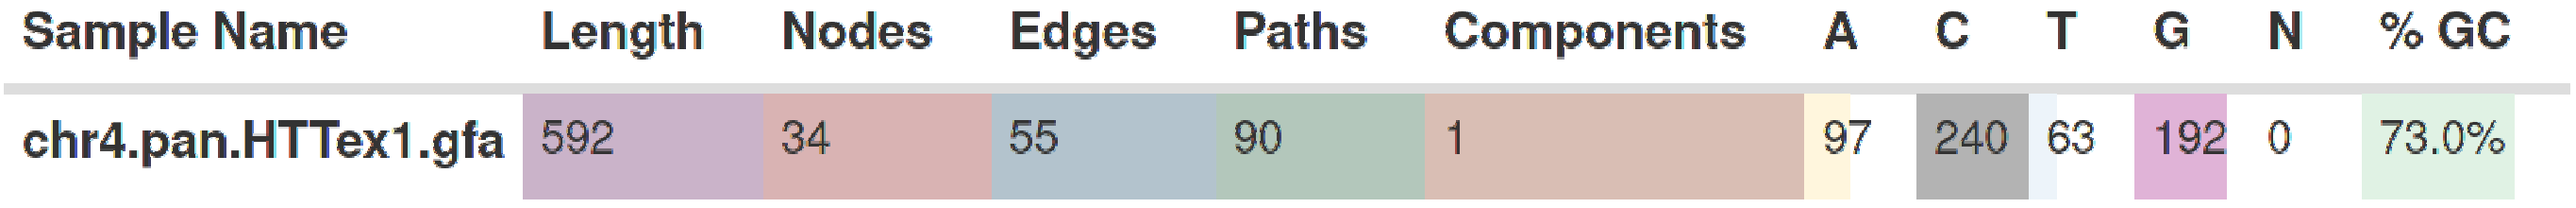
\includegraphics[width=1.0\linewidth, trim=-2.25cm 1.0cm 0cm 3.75cm]{fig/metrics/chr4_pan_HTTex1_gfa_multiqc_odgi_stats_svg}
        \label{fig:metrics-multiqc}
        	\vspace{-2em}
    \end{subfigure}
    \begin{subfigure}{1\linewidth}
        \caption{}
        \centering
        % include fourth image
        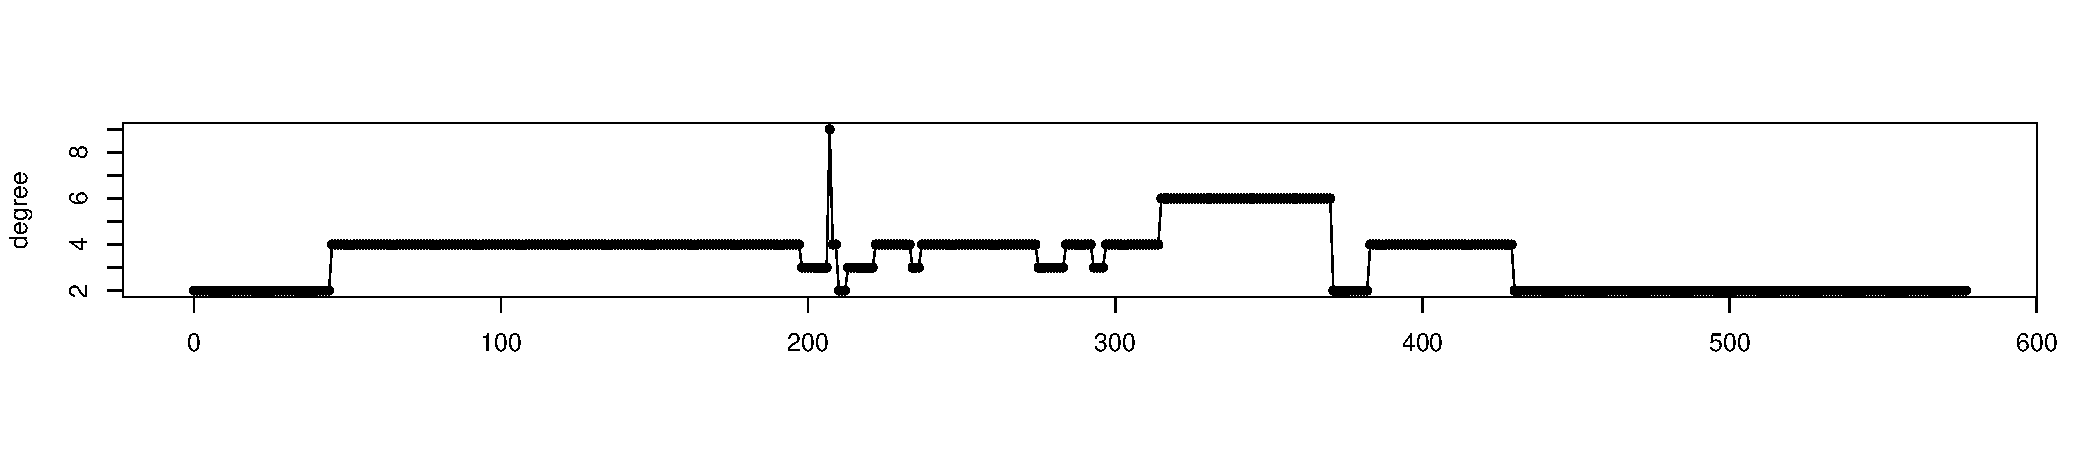
\includegraphics[width=\linewidth,trim=-.225cm 4cm +.425cm +3cm]{fig/metrics/chr4_HTT_chm13_degree_w1_bed}
        \label{fig:metrics-degree}
    \end{subfigure}
    \begin{subfigure}{\linewidth}
        \caption{}
        \centering
        % include second image
        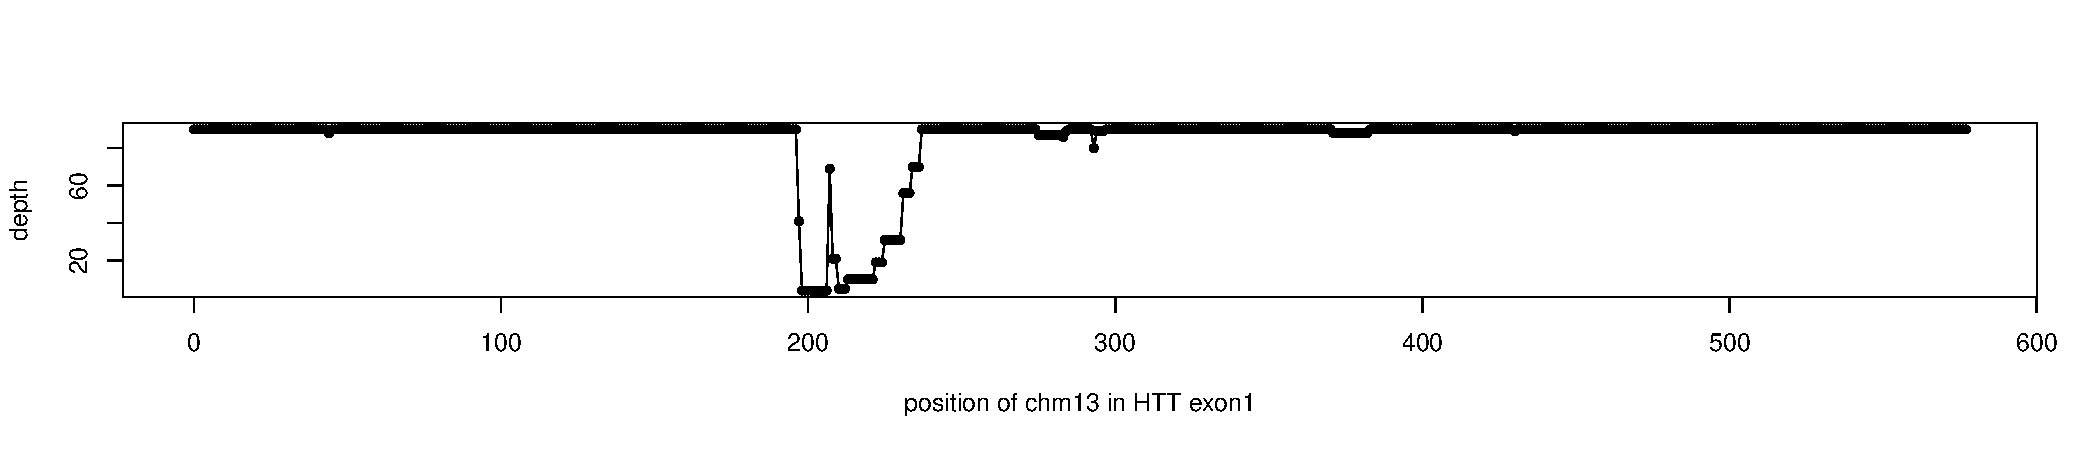
\includegraphics[width=\linewidth,trim=-.225cm 3.3cm +0.425cm +3cm]{fig/metrics/chr4_HTT_chm13_depth_w1_bed}
        \label{fig:metrics-depth}
    \end{subfigure}
    \begin{subfigure}{\linewidth}
        \caption{}
        \centering
        % include second image
        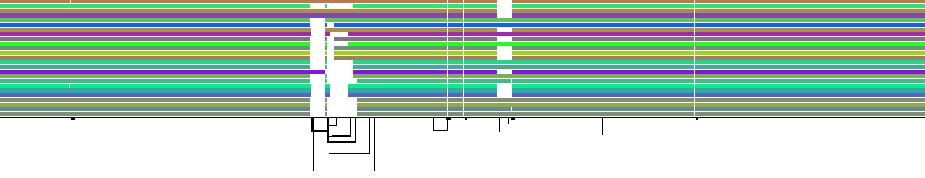
\includegraphics[width=1.0\linewidth, trim=-1.75cm 2.2cm -0.75cm 0.5cm]{fig/metrics/chr4_pan_fa_a2fb268_4030258_6a1ecc2_smooth_gfa_og_HTTex1_og_O_og_tiny_og_png_svg.pdf}
        \label{fig:metrics-viz}
    \end{subfigure}
    \begin{subfigure}{\linewidth}
        \caption{}
        \centering
        % include second image
        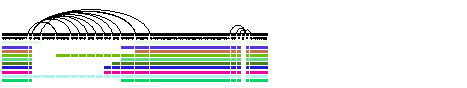
\includegraphics[width=1.0\linewidth, trim=-0.4cm 0.4cm 3.15cm 0cm]{fig/metrics/chr4_pan_HTTex1_STR_xg_svg}
        \label{fig:metrics-str}
        \vspace{-0.5em}
    \end{subfigure}
%	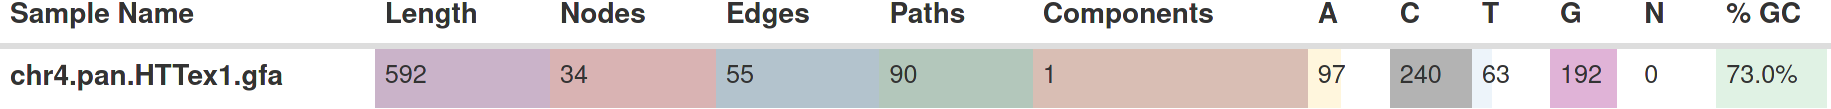
\includegraphics[width=\linewidth]{fig/metrics/chr4.pan.HTTex1.gfa.multiqc_odgi_stats.png}
	\caption{Features of a 90-haplotype human pangenome graph of the exon 1 huntingtin gene (\textit{HTTexon1}): \textbf{(a)} Excerpt of vital statistics of the \textit{HTTexon1} graph displayed by MultiQC's ODGI module. The very high GC content of 73.0\% compared to a human genomic mean GC content of 40.9\% \citep{Piovesan2019} is in accordance with the literature \citep{Neueder2017}. \textbf{(b)} Per nucleotide node degree distribution of CHM13 in the \textit{HTTexon1} graph. Around position 200 there is a huge variation in node degree. \textbf{(c)} Per nucleotide node depth distribution of CHM13 in the \textit{HTTexon1} graph. The alternating depth around position 200 indicates polymorphic variation complementing the above node degree analysis. \textbf{(d)} \textit{odgi viz} visualization of the 23 largest gene alleles, CHM13, and GRCH38 of the \textit{HTTexon1} graph. \textbf{(e)} \textit{vg viz} nucleotide-level visualization of 10 gene alleles, CHM13, GRCH38 of the \textit{HTTexon1} graph focusing on the CAG variable repeat region. Figures \textbf{(b)-(e)} highlight the variant region around position 200 of CHM13 showing the variable number of glutamine residues of the different individuals as reported by \citep{Nance1999}.}
	\label{fig:metrics}
\end{figure}


% Figure: small graph with all the stats shown. A screenshot of MultiQC, visualize summary per bin somehow, R visualizations of degree and depth HTT exon 1 as tiny example graph


\section{Discussion}

% erik & pjotr & anyone

Pangenome graphs stand to become a ubiquitous tool in genomics \citep{Eizenga_2020}. With ODGI we implemented a state-of-the-art tool suite that can transform, analyse, simplify, validate, and visualise pangenome graphs at large scale. Lifting over annotations and linearizing nested graph structures place the suite as the bridge between traditional linear reference genome analysis and pangenome graphs. ODGI is a unique set of tools that enables scientists to explore and discover the underlying biology of pangenome graphs. Already, the tools are the backbone of pipelines such as the Pangenome Graph Builder\footnote{\url{https://github.com/pangenome/pggb} (accessed Oct 2021)} (PGGB) or nf-core/pangenome\footnote{\url{https://github.com/nf-core/pangenome} (accessed Oct 2021)}. Future work will add support for RNA and protein sequences and expand on metadata capabilities of large pangenome graphs.

rdf sparql side, bring in annotation for great biological interpretation \cite{Yokoyama2020}, federated queries, sharing, FAIR

(recent) interactive visualization tools?! CITE PANACHE, also indicate that no published tool for interactive exploration of such graphs exist
\FIXME{mention gfaestus?}

is ODGI ready for scWGS data? potentially, each cell is a path in a graph!! very very high path depth

some cancer stuff?!

\FIXME{I think we can leave RDF and FAIR out as it does not really relate to performance and ODGI explorations. Cancer, yes, we could state that the tools are applicable to cancer genome exploration as wild variation can be represented :)}

\section*{Funding}

S.H. acknowledges funding from the Central Innovation Programme (ZIM) for SMEs of the Federal Ministry for Economic Affairs and Energy of Germany.
This work was supported by the BMBF-funded de.NBI Cloud within the German Network for Bioinformatics Infrastructure (de.NBI) (031A537B, 031A533A, 031A538A, 031A533B, 031A535A, 031A537C, 031A534A, 031A532B).

\section*{Data availability}

Data used to build Human pangenome graphs is available at \url{https://github.com/human-pangenomics/HPP_Year1_Data_Freeze_v1.0}.
TODO!

\bibliographystyle{natbib}
%\bibliographystyle{achemnat}
%\bibliographystyle{plainnat}
%\bibliographystyle{abbrv}
%\bibliographystyle{bioinformatics}
%
%\bibliographystyle{plain}
%
\bibliography{document}


% \begin{thebibliography}{}

% \bibitem[Bofelli {\it et~al}., 2000]{Boffelli03}
% Bofelli,F., Name2, Name3 (2003) Article title, {\it Journal Name}, {\bf 199}, 133-154.

% \bibitem[Bag {\it et~al}., 2001]{Bag01}
% Bag,M., Name2, Name3 (2001) Article title, {\it Journal Name}, {\bf 99}, 33-54.

% \bibitem[Yoo \textit{et~al}., 2003]{Yoo03}
% Yoo,M.S. \textit{et~al}. (2003) Oxidative stress regulated genes
% in nigral dopaminergic neurnol cell: correlation with the known
% pathology in Parkinson's disease. \textit{Brain Res. Mol. Brain
% Res.}, \textbf{110}(Suppl. 1), 76--84.

% \bibitem[Lehmann, 1986]{Leh86}
% Lehmann,E.L. (1986) Chapter title. \textit{Book Title}. Vol.~1, 2nd edn. Springer-Verlag, New York.

% \bibitem[Crenshaw and Jones, 2003]{Cre03}
% Crenshaw, B.,III, and Jones, W.B.,Jr (2003) The future of clinical
% cancer management: one tumor, one chip. \textit{Bioinformatics},
% doi:10.1093/bioinformatics/btn000.

% \bibitem[Auhtor \textit{et~al}. (2000)]{Aut00}
% Auhtor,A.B. \textit{et~al}. (2000) Chapter title. In Smith, A.C.
% (ed.), \textit{Book Title}, 2nd edn. Publisher, Location, Vol. 1, pp.
% ???--???.

% \bibitem[Bardet, 1920]{Bar20}
% Bardet, G. (1920) Sur un syndrome d'obesite infantile avec
% polydactylie et retinite pigmentaire (contribution a l'etude des
% formes cliniques de l'obesite hypophysaire). PhD Thesis, name of
% institution, Paris, France.

% \end{thebibliography}
\end{document}
